\section{Umsetzung des Hopfield-Netzwerks in Simulink}
\label{app:Umsetzung des Hopfield-Netzwerks in Simulink}

Ein \gls{hopfieldnetzwerk} mit zwei Neuronen wurde nach der von \cite{Scellier2017} vorgestellten Dynamik in Simulink modelliert und ist in Abbildung \ref{fig:Hopfield-Netzwerk 2 Neuronen Simulink} dargestellt.

\begin{figure}[h]
  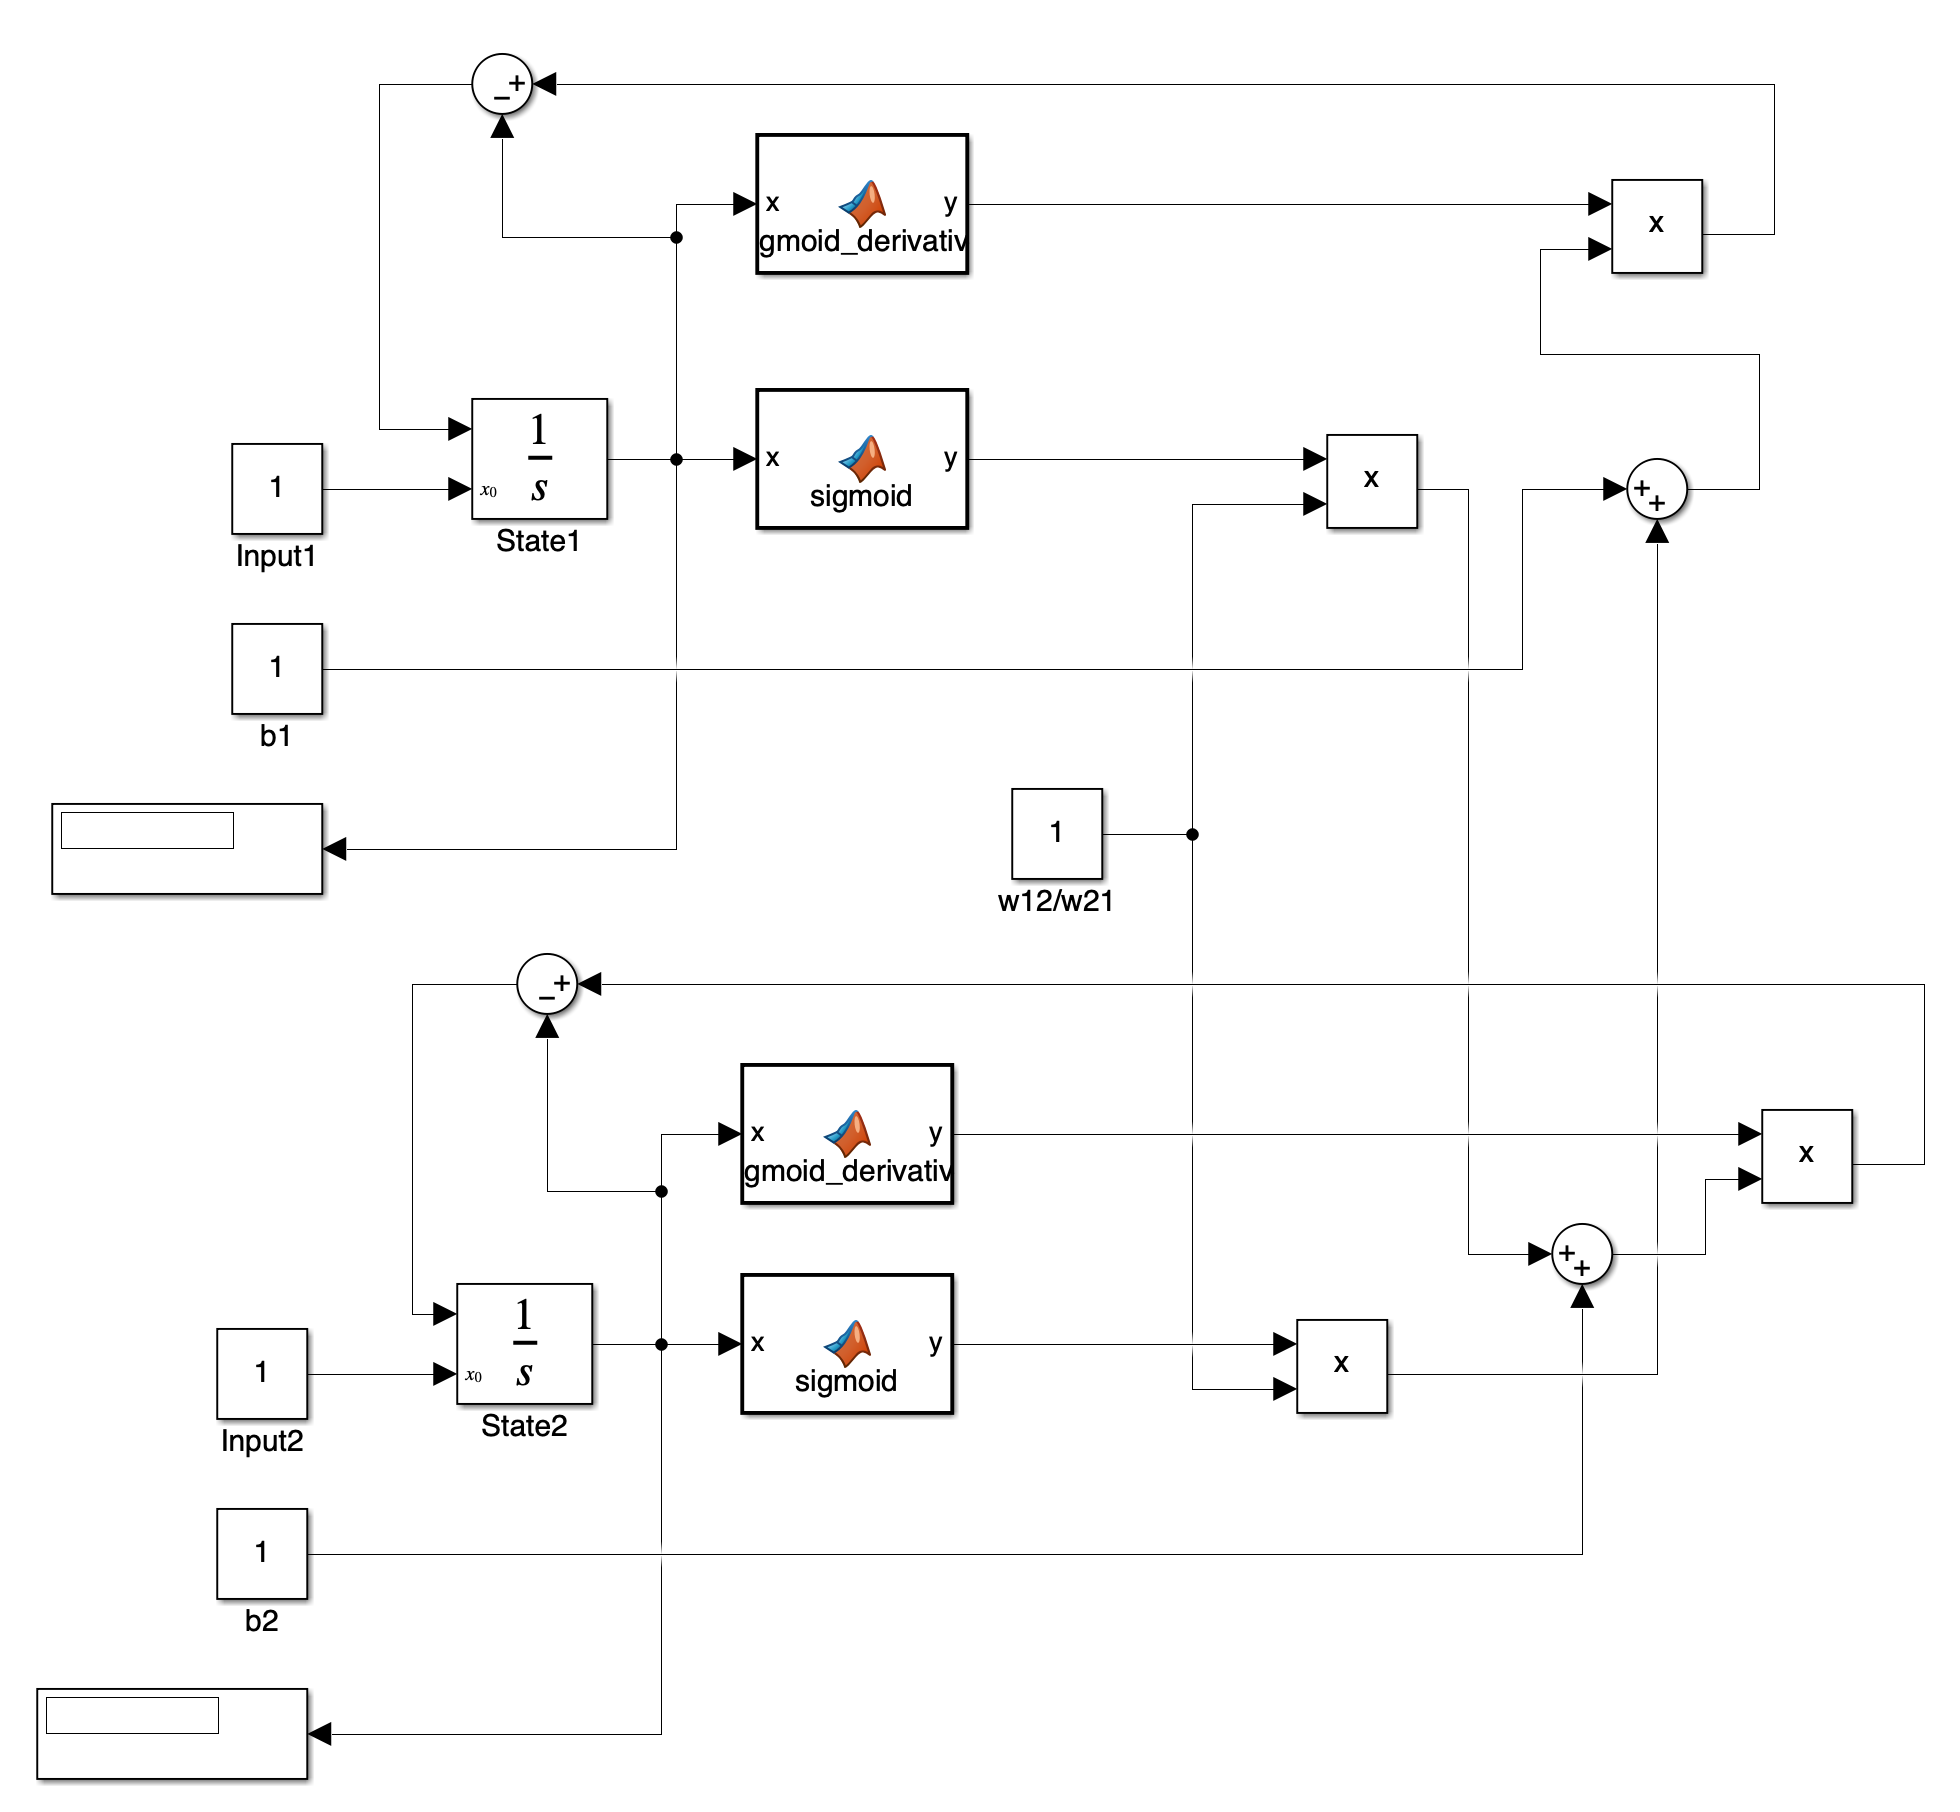
\includegraphics[width=\textwidth]{abbildungen/hnn_2_neurons_simulink.png}
  \caption{Umsetzung eines \gls{hopfieldnetzwerk}s mit zwei Neuronen in Simulink. Quelle: \textit{Eigene Darstellung}}
  \label{fig:Hopfield-Netzwerk 2 Neuronen Simulink}
\end{figure}

Ein auf drei Neuronen skaliertes Modell ist in Abbildung \ref{fig:Hopfield-Netzwerk 3 Neuronen Simulink} dargestellt. Hier wurde auch die Kostenfunktion des \gls{eqprop} umgesetzt, nur der Bias wurde zur Übersichtlichkeit weggelassen.

\begin{figure}[h]
  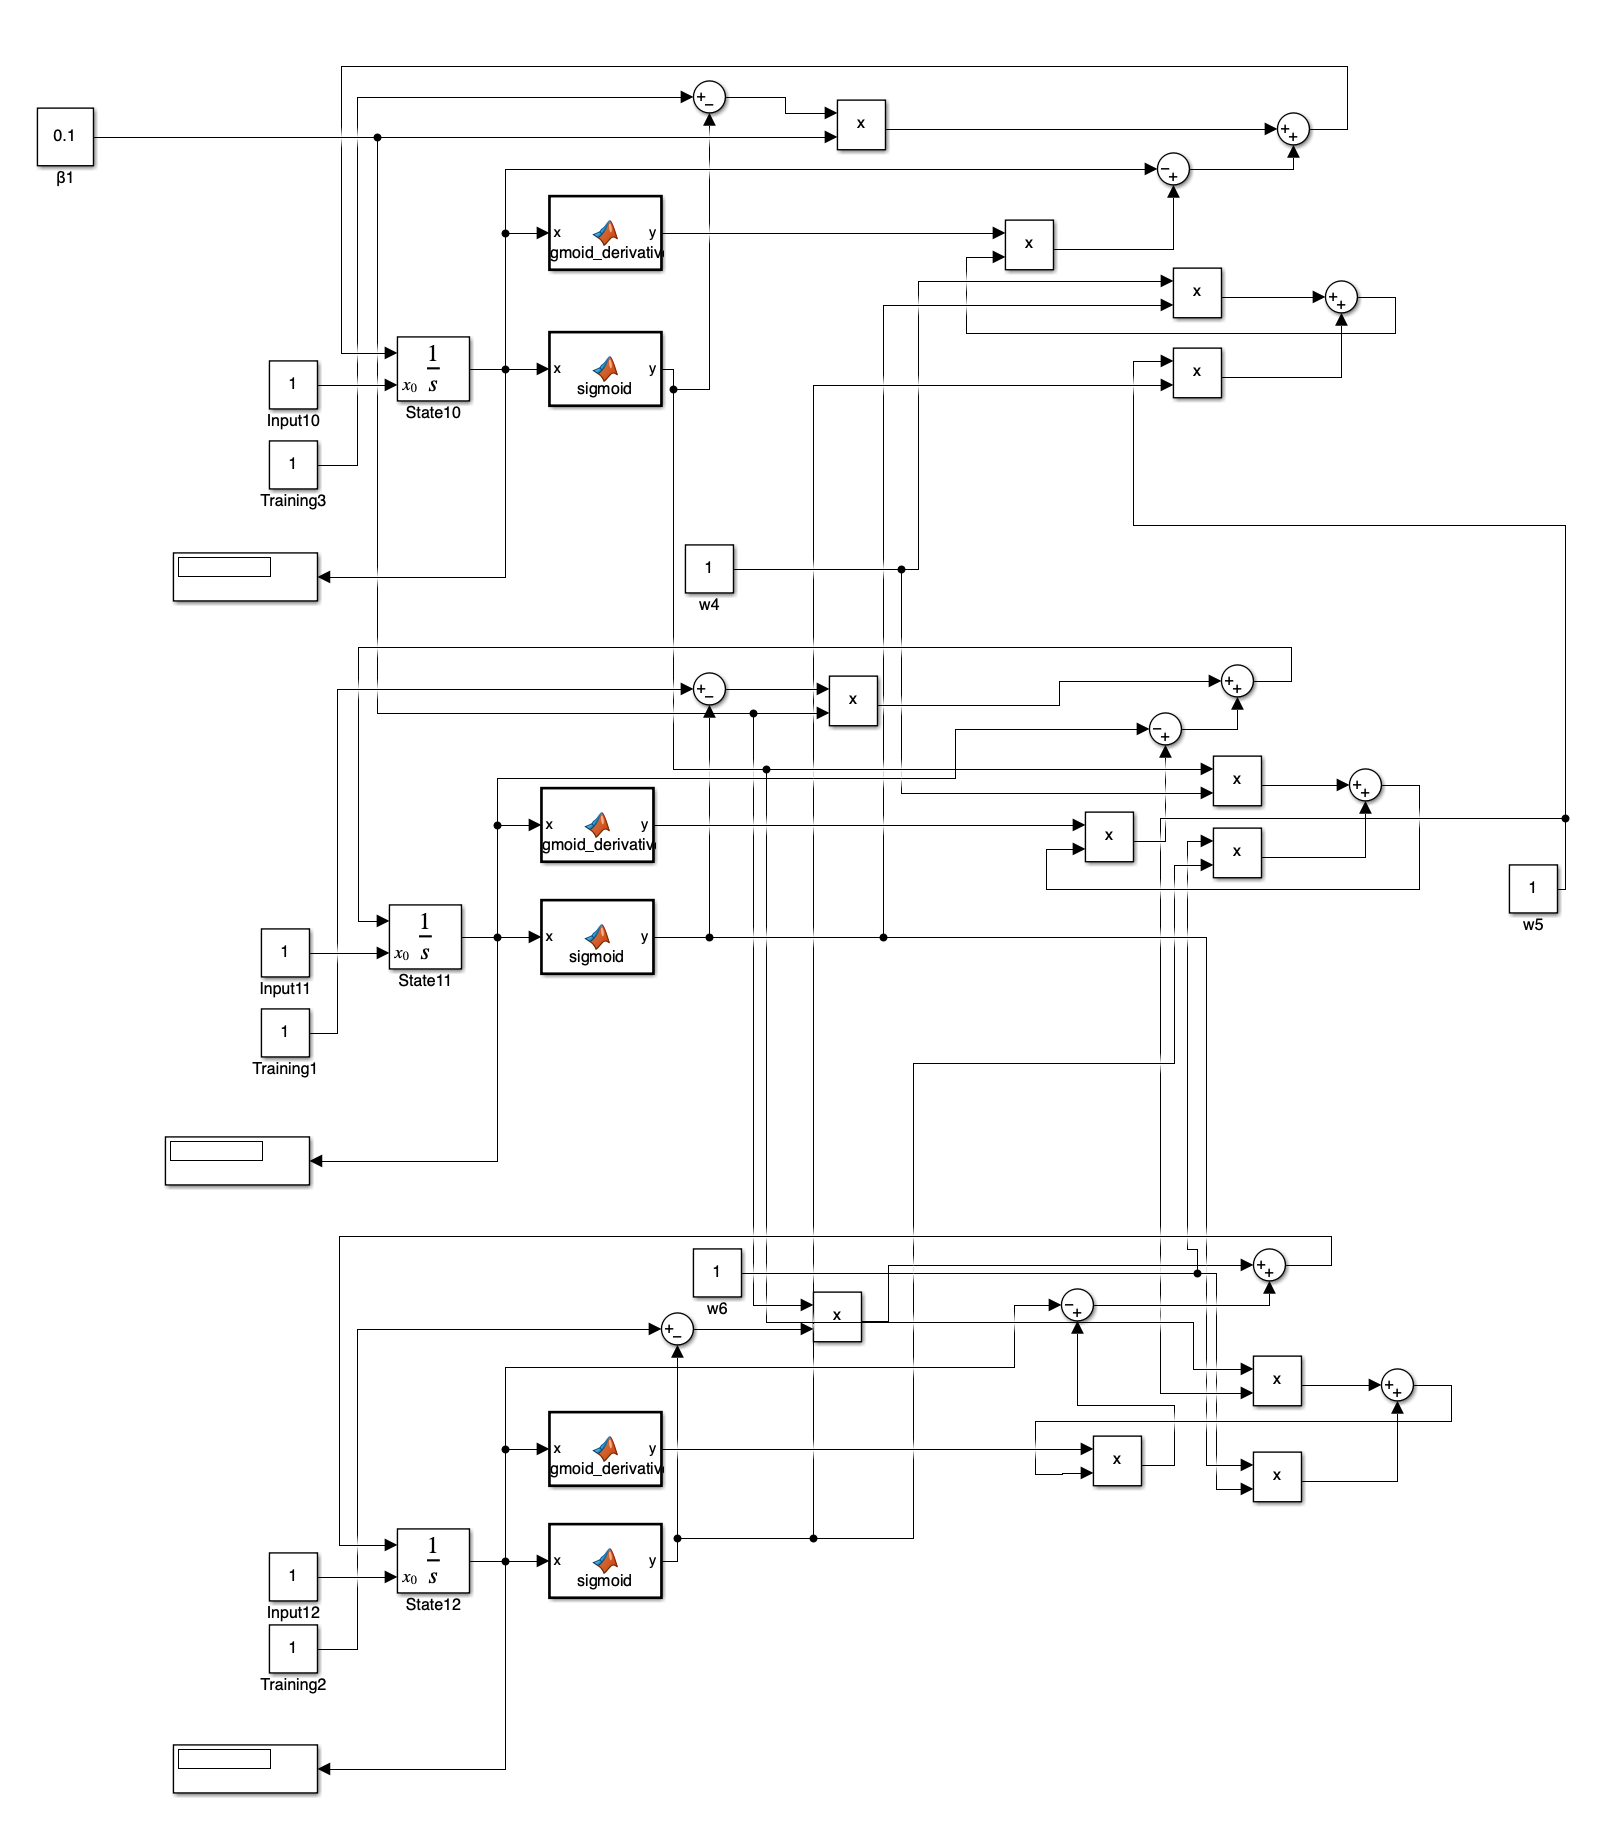
\includegraphics[width=\textwidth]{abbildungen/hnn_without_bias_with_cost_3_neurons_simulink.png}
  \caption{Umsetzung eines \gls{hopfieldnetzwerk}s mit drei Neuronen in Simulink. Quelle: \textit{Eigene Darstellung}}
  \label{fig:Hopfield-Netzwerk 3 Neuronen Simulink}
\end{figure}

Zur Vereinfachung der Arbeit mit dem \gls{hopfieldnetzwerk} in Simulink wurde dieses für die Nutzung von Vektoren und Matrizen umgeformt, wie in Abbildung \ref{fig:Hopfield-Netzwerk Final Simulink} dargestellt. Die Gewichte sind als Integratoren für skalare Werte vorhanden und werden über einen Matlab-Funktionsblock zu einer Gewichtsmatrix umgeformt.

Anhand des Funktionsblocks "`dynamics"' unterhalb des Netzwerks kann die Funktionsweise dessen validiert werden. Da die Ausgaben "`Output"' und "`Output1"' übereinstimmen, wird gezeigt, dass das \gls{hopfieldnetzwerk} eine korrekte Analogie zur Dynamik \(\frac{ds}{dt}\) darstellt.

\begin{figure}[h]
  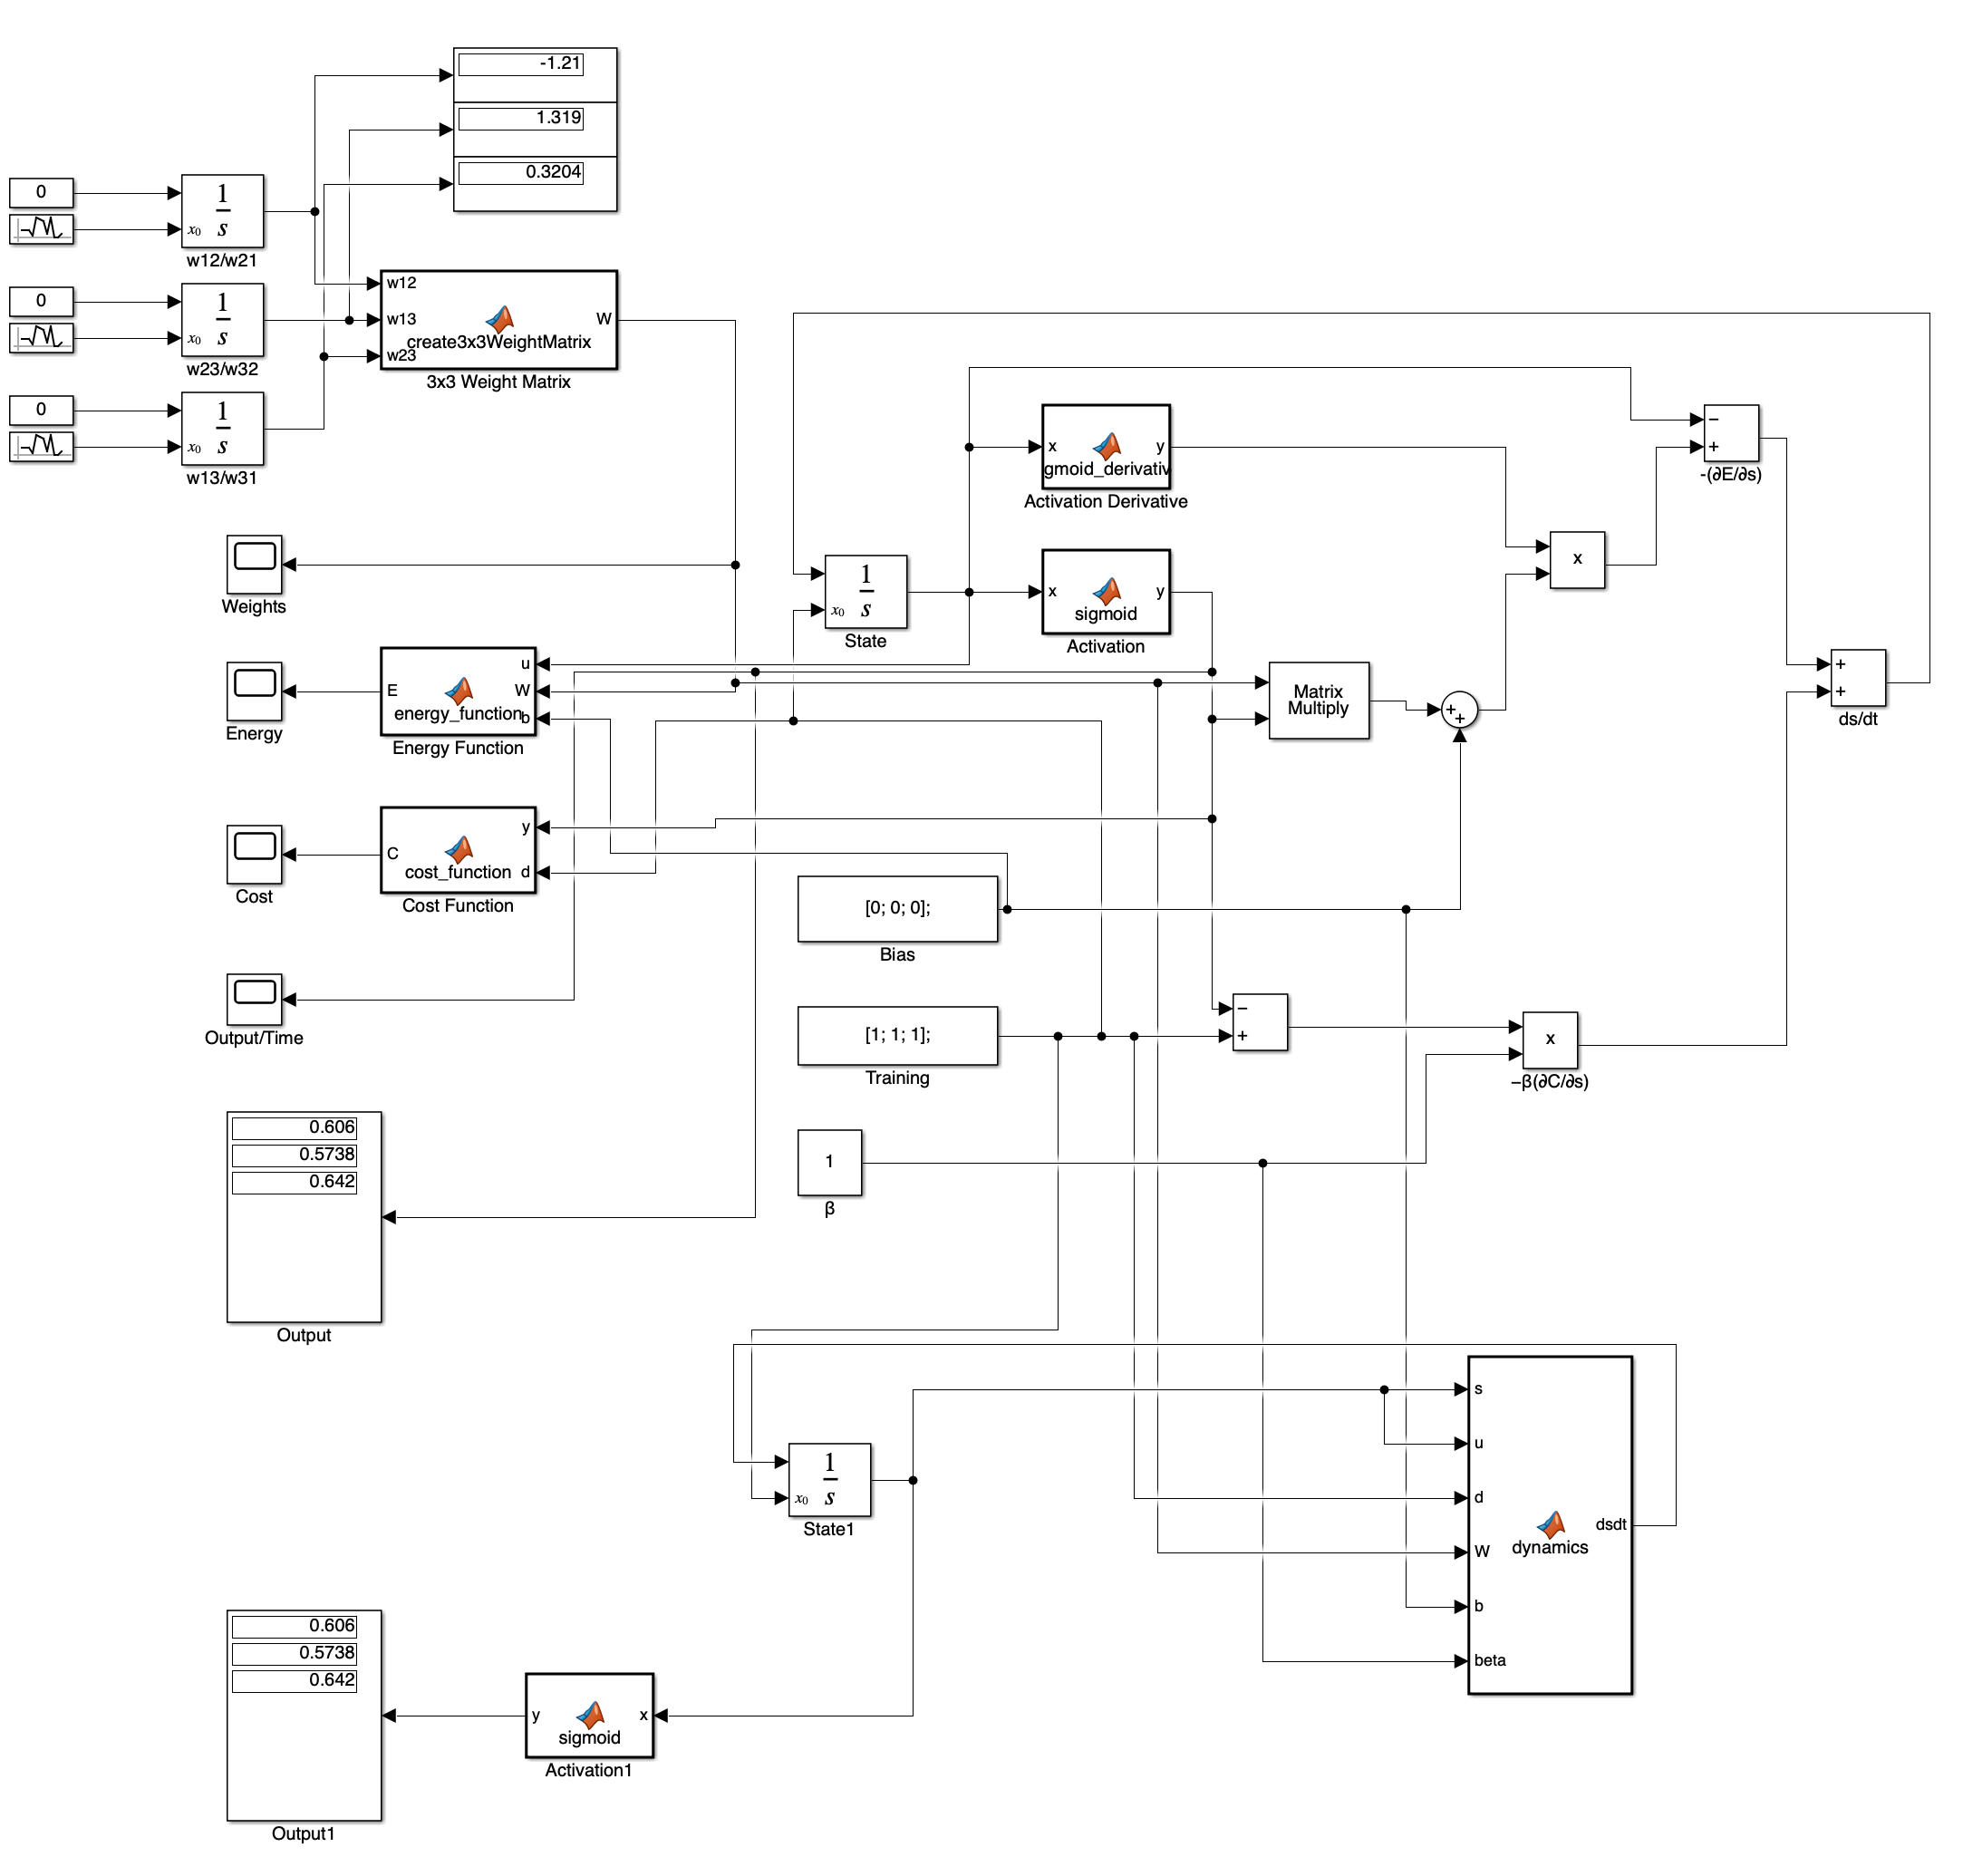
\includegraphics[width=\textwidth]{abbildungen/hnn_with_proof_simulink.png}
  \caption{Finales Modell des \gls{hopfieldnetzwerk} in Simulink mit einem Funktionsblock zur Validierung der Funktionsweise. Quelle: \textit{Eigene Darstellung}}
  \label{fig:Hopfield-Netzwerk Final Simulink}
\end{figure}

Es folgt der Quellcode für die Funktionsblöcke "`dynamics"', "`sigmoid"' und "`sigmoid derivative"' sowie zur Erstellung der Gewichtsmatrix.

\lstinputlisting[language=Octave]{./Quellcode/hopfield_netzwerk_dynamik.m}
\lstinputlisting[language=Octave]{./Quellcode/sigmoid.m}
\lstinputlisting[language=Octave]{./Quellcode/sigmoid_derivative.m}
\lstinputlisting[language=Octave]{./Quellcode/weight_matrix.m}
